\chapter{Strain-Stress-Resistance Experiments}
\label{appendix-B}
%\section{title}
\begin{figure}[H]
	\centering
	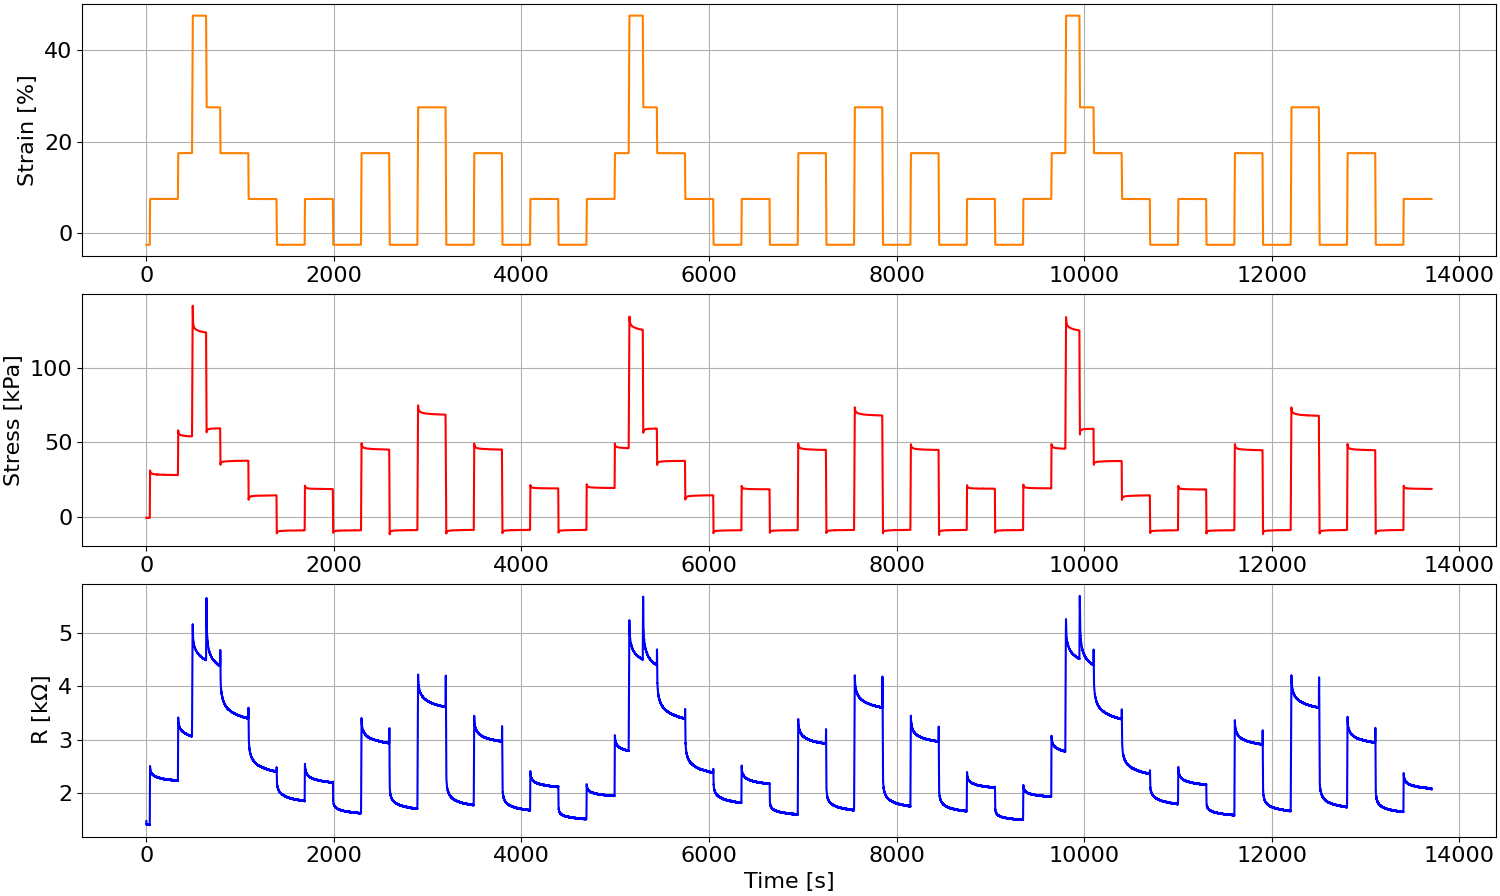
\includegraphics[width=\linewidth]{Figures/2_7-5_E4pin_20mm_v12_0.1_0.2_0.3_strain_1mm_offset_erroneous.png}
	\caption{Strain test sequence showing the shoulder phenomena correlation for varying magnitudes of strain for a 7.5 wt\% CBSR specimen dogbone sample. This experiment had an unintentional offset of 1 mm, however this showed a drastic decrease shoulder phenomena when the falling edge is crossing the x-axis.}
	\label{fig:strain-hill}
\end{figure}
\begin{figure}[H]
	\centering
	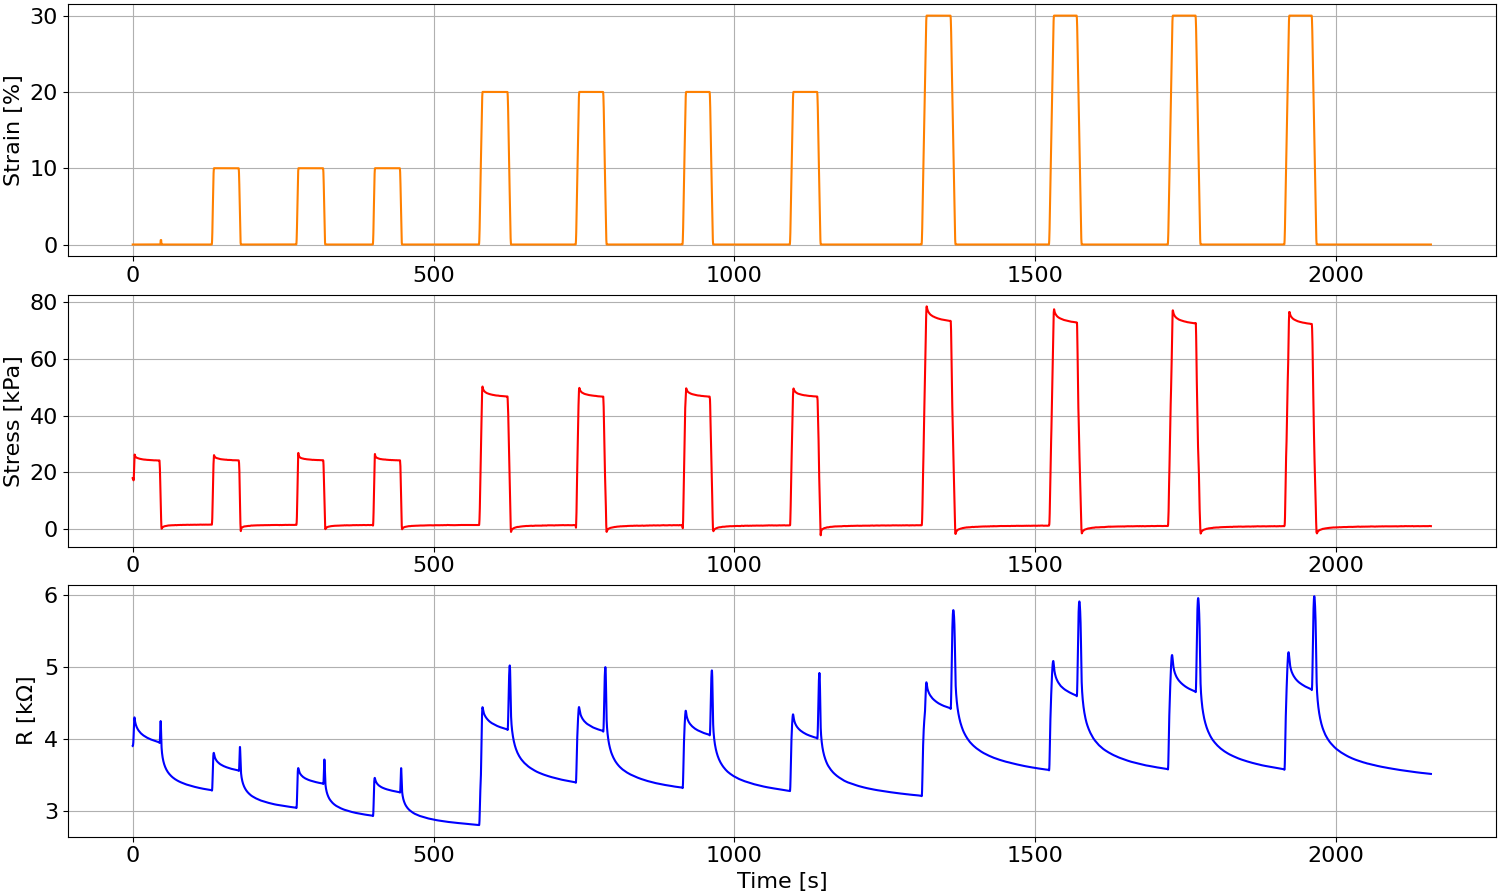
\includegraphics[width=\linewidth]{Figures/1_7-5_Epin_20mm_v2_DC_meas_3_strains.png}
	\caption{Strain test sequence showing the shoulder phenomena correlation for varying magnitudes of strain for a 7.5 wt\% CBSR specimen dogbone sample. This experiment used DC measurements, so the macro downward trend in resistance is more obvious than other experimental data given in this work with used a switched AC signal.}
	\label{fig:strain-train-DC-meas}
\end{figure}
\begin{figure}[H]
	\centering
	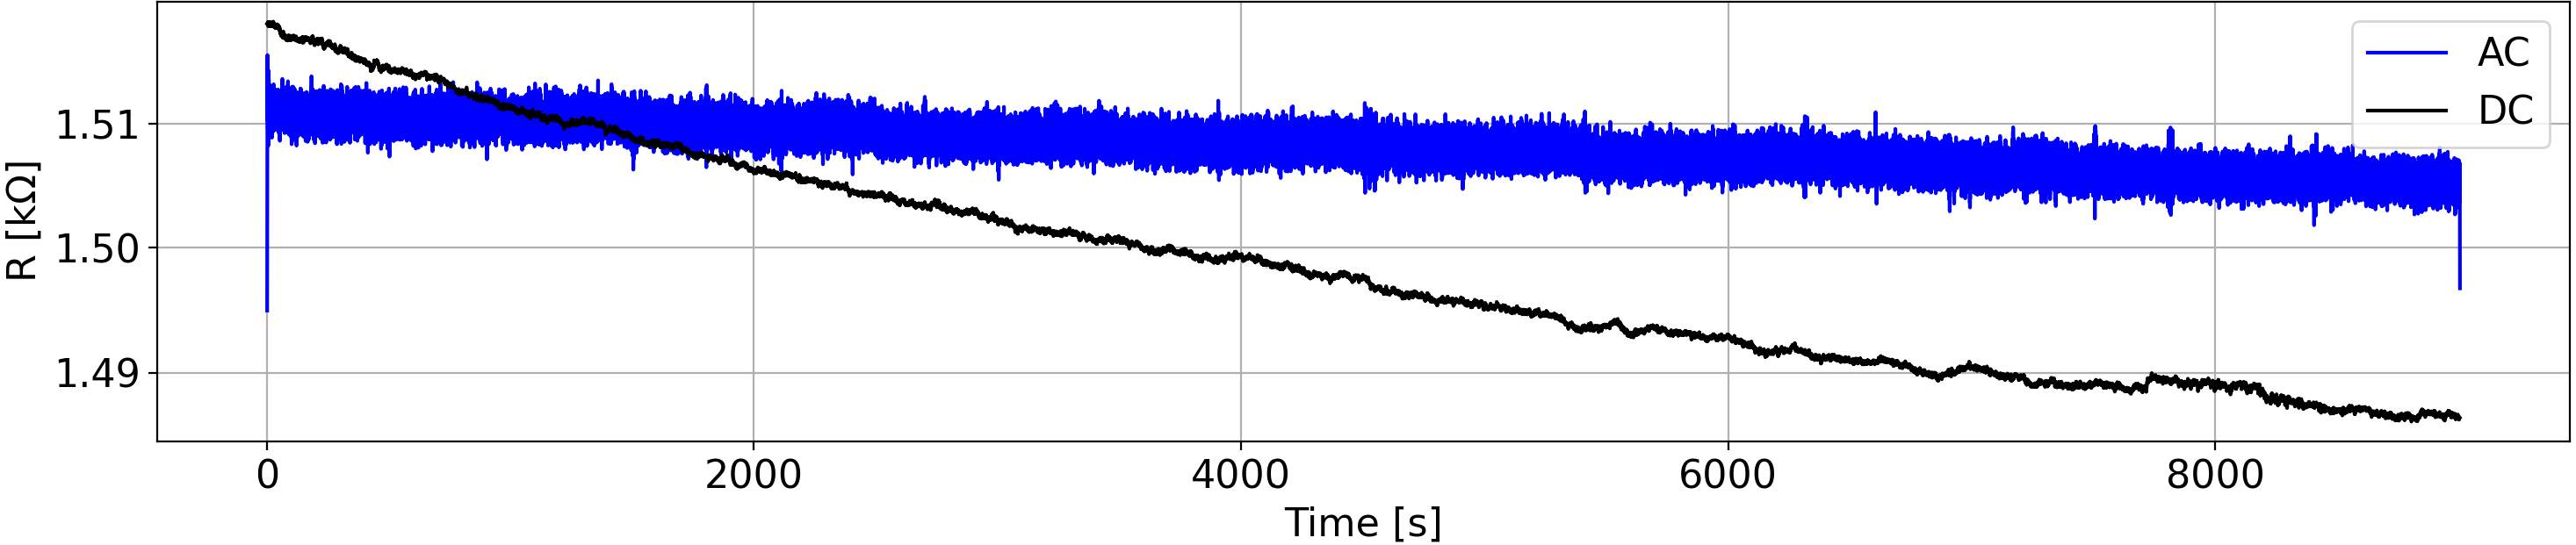
\includegraphics[width=\linewidth]{Figures/AC_vs_DC_long_decay_2_7-5_CBSR}
	\caption{AC vs DC downward trend in resistance for an unstrained 7.5 wt\% CBSR composite dogbone specimen.}
	\label{fig:res-AC-DC}
\end{figure}

